% Figure 1: Dual-Process System Architecture
% Standalone compilable: pdflatex fig1_architecture.tex
\documentclass[border=5pt]{standalone}
\usepackage{tikz}
\usetikzlibrary{shapes.geometric, arrows.meta, positioning, fit, backgrounds, calc}

\begin{document}
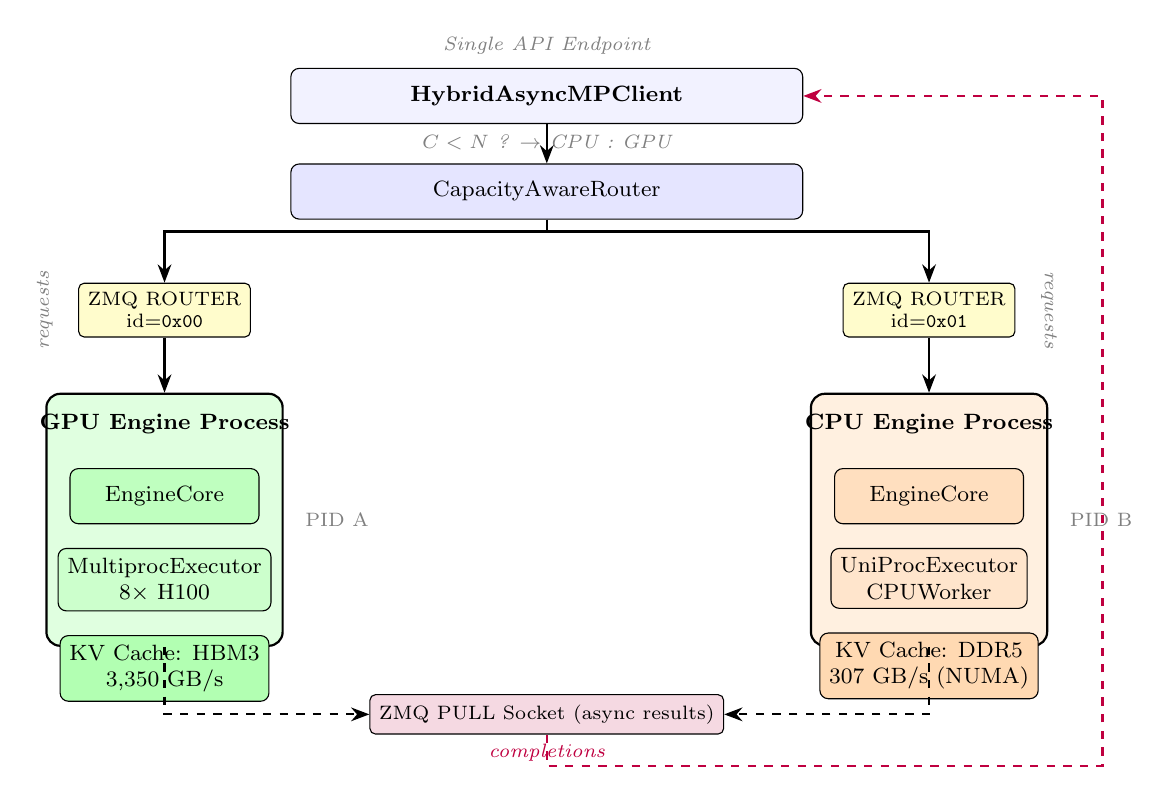
\begin{tikzpicture}[
    >=Stealth,
    node distance=0.6cm,
    box/.style={draw, rounded corners=3pt, minimum width=2.2cm, minimum height=0.7cm, align=center, font=\footnotesize},
    bigbox/.style={draw, rounded corners=5pt, thick, minimum width=2.8cm, align=center, font=\footnotesize},
    label/.style={font=\scriptsize\itshape, text=gray},
    sock/.style={draw, fill=yellow!20, rounded corners=2pt, minimum width=1.8cm, minimum height=0.5cm, align=center, font=\scriptsize},
    arrow/.style={->, thick},
    darrow/.style={<->, thick},
  ]

  % --- Router Layer ---
  \node[box, fill=blue!10, minimum width=6.5cm, minimum height=0.7cm] (router) {CapacityAwareRouter};
  \node[label, above=0.05cm of router] {$C < N$ ? $\to$ CPU : GPU};

  \node[box, fill=blue!5, minimum width=6.5cm, minimum height=0.7cm, above=0.5cm of router] (client) {\textbf{HybridAsyncMPClient}};
  \node[label, above=0.05cm of client] {Single API Endpoint};

  % --- ZMQ Sockets ---
  \node[sock, below left=0.8cm and 0.5cm of router] (zmq_gpu) {ZMQ ROUTER\\id=\texttt{0x00}};
  \node[sock, below right=0.8cm and 0.5cm of router] (zmq_cpu) {ZMQ ROUTER\\id=\texttt{0x01}};

  % --- GPU Engine ---
  \node[bigbox, fill=green!12, below=0.7cm of zmq_gpu, minimum height=3.2cm, minimum width=3.0cm] (gpu_outer) {};
  \node[font=\footnotesize\bfseries, anchor=north] at ([yshift=-0.15cm]gpu_outer.north) {GPU Engine Process};
  \node[box, fill=green!25, minimum width=2.4cm] at ([yshift=0.3cm]gpu_outer.center) (gpu_core) {EngineCore};
  \node[box, fill=green!20, minimum width=2.4cm, below=0.3cm of gpu_core] (gpu_exec) {MultiprocExecutor\\8$\times$ H100};
  \node[box, fill=green!30, minimum width=2.4cm, below=0.3cm of gpu_exec] (gpu_kv) {KV Cache: HBM3\\3,350 GB/s};

  % --- CPU Engine ---
  \node[bigbox, fill=orange!12, below=0.7cm of zmq_cpu, minimum height=3.2cm, minimum width=3.0cm] (cpu_outer) {};
  \node[font=\footnotesize\bfseries, anchor=north] at ([yshift=-0.15cm]cpu_outer.north) {CPU Engine Process};
  \node[box, fill=orange!25, minimum width=2.4cm] at ([yshift=0.3cm]cpu_outer.center) (cpu_core) {EngineCore};
  \node[box, fill=orange!20, minimum width=2.4cm, below=0.3cm of cpu_core] (cpu_exec) {UniProcExecutor\\CPUWorker};
  \node[box, fill=orange!30, minimum width=2.4cm, below=0.3cm of cpu_exec] (cpu_kv) {KV Cache: DDR5\\307 GB/s (NUMA)};

  % --- PULL Socket ---
  \node[sock, fill=purple!15, below=0.6cm of $(gpu_outer.south)!0.5!(cpu_outer.south)$, minimum width=3.5cm] (zmq_pull) {ZMQ PULL Socket (async results)};

  % --- Arrows: Client to Router ---
  \draw[arrow] (client) -- (router);

  % --- Arrows: Router to ZMQ ---
  \draw[arrow] (router.south) -- ++(0,-0.15) -| (zmq_gpu.north);
  \draw[arrow] (router.south) -- ++(0,-0.15) -| (zmq_cpu.north);

  % --- Arrows: ZMQ to Engines ---
  \draw[arrow] (zmq_gpu.south) -- (gpu_outer.north);
  \draw[arrow] (zmq_cpu.south) -- (cpu_outer.north);

  % --- Arrows: Engines to PULL ---
  \draw[arrow, dashed] (gpu_outer.south) |- (zmq_pull.west);
  \draw[arrow, dashed] (cpu_outer.south) |- (zmq_pull.east);

  % --- Arrow: PULL back to Client ---
  \draw[arrow, dashed, color=purple] (zmq_pull.south) -- ++(0,-0.4) -| ([xshift=3.8cm]client.east) -- (client.east);

  % --- Labels on arrows ---
  \node[label, rotate=90, anchor=south] at ([xshift=-0.2cm]zmq_gpu.west) {requests};
  \node[label, rotate=270, anchor=south] at ([xshift=0.2cm]zmq_cpu.east) {requests};
  \node[label, anchor=north] at (zmq_pull.south) {\textcolor{purple}{completions}};

  % --- Process isolation labels ---
  \node[font=\scriptsize, text=gray, anchor=west] at ([xshift=0.15cm]gpu_outer.east) {PID A};
  \node[font=\scriptsize, text=gray, anchor=west] at ([xshift=0.15cm]cpu_outer.east) {PID B};

\end{tikzpicture}
\end{document}
